\chapter{Experimentelle Untersuchungen im Windkanal}
\label{s:versuche}
%%%%%%%%%%%%%%%%%%%%%%%%Modellbeschreibung Tim%%%%%%%%%%%%%%%%%%%%%%%%%%%%%
\section{Das Versuchsmodell (TG)}
\label{sec:Modell}
Die Versuche werden am gleichen Modell duchgef"uhrt, welches im Zuge der Arbeit von Bilges \cite{Bilges.2018} verwendet wurde. Die Form entstammt der Arbeit von Oswald \cite{Oswald.2017}. Eine Skizze des Modells ist in \abb{fig:SkizzeModell} zu sehen.

\begin{figure}[h]
	\centering
	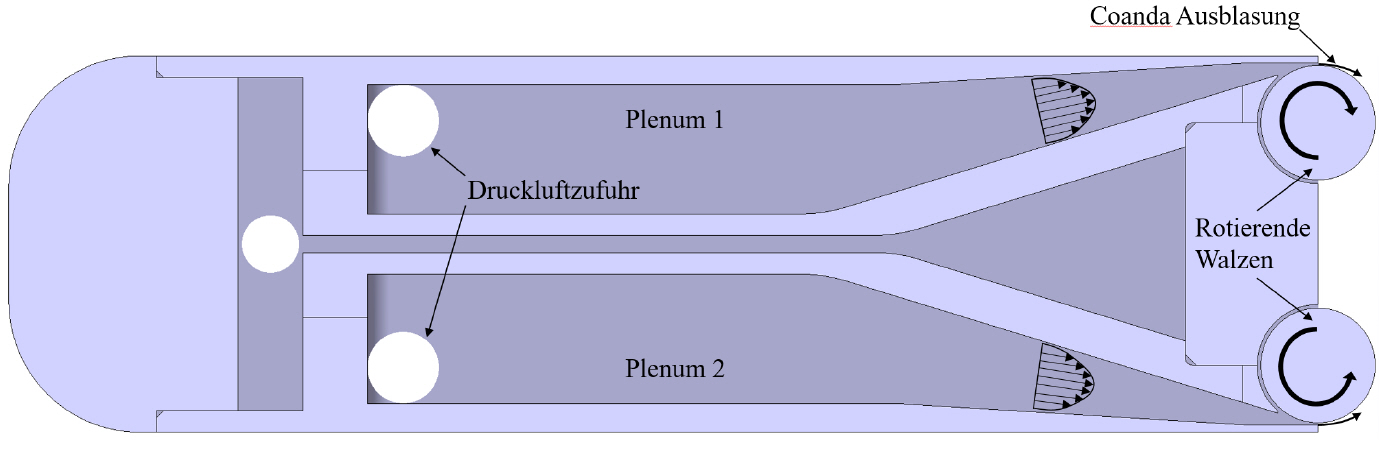
\includegraphics[width=0.9\textwidth]{SkizzeModell.jpg}
	\caption{Skizze des Versuchsmodells \citep{Bilges.2018}}
	\label{fig:SkizzeModell}
\end{figure}

Im Inneren teilt sich der Stumpfk"orper in zwei Kammern auf, welche mit Plenum 1 und Plenum 2 an der Ober- respektive Unterseite des K"orpers bezeichnet sind. "Uber die eingezeichneten "Offnungen im vorderen Teil werden die beiden Plenen "uber 4 Druckluftschl"auche mit bis zu 8 bar Druckluft versorgt, wobei diese in den Hinterteil des K"orpers str"omt. Hier findet durch den eingezeichneten Spalt eine Coand\^{a}-Ausblasung "uber die entgegengesetzt rotierenden Walzen aus Kapitel \ref{s:rotierendeWalzen} statt.

Zur Bestimmung der Oberfl"achendr"ucke sind entlang der K"orperkontur mittig an der Ober- und Unterseite 32 Druckluftbohrungen platziert worden. Die Position der Bohrungen sowie die folgend beschriebene Geometrie des K"orpers ist in \abb{fig:ModellGeometrie} ersichtlich. Das Modell kann als D-Stumpfk"orper klassifiziert werden und hat folgende Abmessungen: 
\begin{center}
H"ohe: h = 53,4 mm\\
Breite: b = 390 mm\\
L"ange: l = 190,6 mm\\ 
\end{center}
Dabei ist die Breite des Modells so gew"ahlt, dass dessen Seiten inklusive Fl"achendichtungen b"undig an der Windkanalwand abschlie\ss{}en. 

\begin{figure}[h]
	\centering
	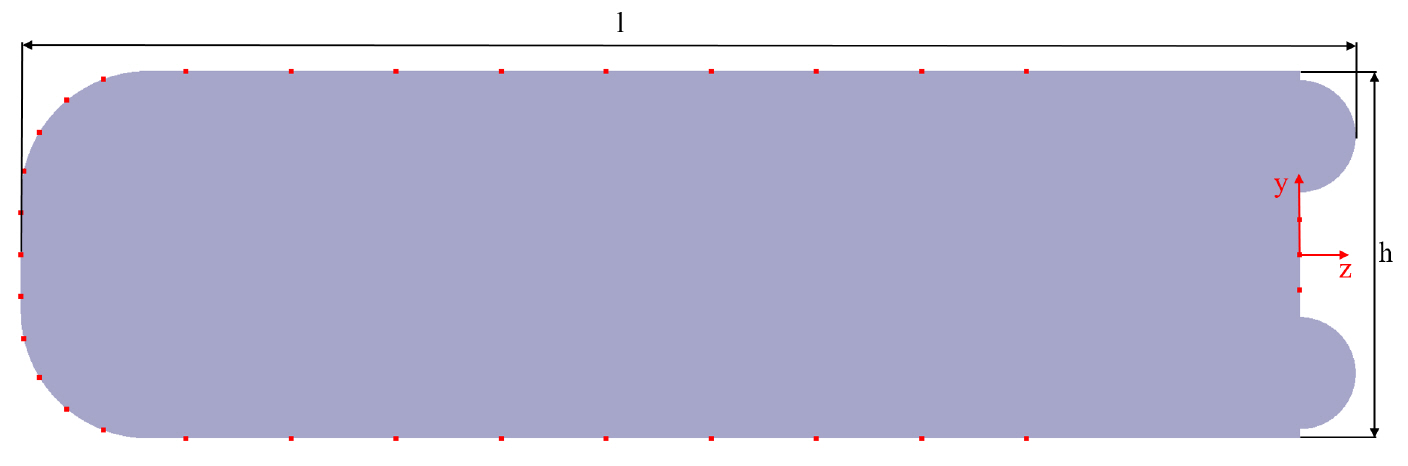
\includegraphics[width=0.75\textwidth]{ModellGeometrie.jpg}
	\caption{Geometrie des D-Stumpfk"orpers mit eingezeichneten Druckbohrungen \citep{Bilges.2018}}
	\label{fig:ModellGeometrie}
\end{figure}

Die oben erw"ahnten Druckmessbohrungen sind in \abb{fig:DModell1} erkennbar. Deren Messschl"auche werden vorne an den Seiten des Modells herausgef"uhrt. Die Aluminiumholme rechts und links dienen zur Aufh"angung und genauen Justierung des Modells innerhalb des Windkanals. Die beidseitig sichtbaren Messinganschl"usse sind die bereits erw"ahnten Anschl"usse f"ur die Druckluft.

Wie schon in Abschnitt \ref{sec:Vorderkante} erl"autert wurde, erzeugt die Vorderkante eine laminare Abl"oseblase, wie es in \abb{fig:LamBlase} dargestellt ist. Um Str"omungsabl"osungen zu vermeiden, wird daher an der Vorderkante des Modells an der Ober- und Unterseite ein Zackenband befestigt. Dieses Band, welches vor der Abl"osezone befestigt wird, dient als Wirbelgenerator und sorgt daf"ur, dass die laminare Str"omung zwangsweise in turbulente Str"omung umgewandelt wird. Auf H"ohe der Abl"oseblase sorgt die Turbulenz zu einem Engergietransport quer zur Anstr"omung, was dazu f"uhrt, dass die Abl"oseblase geschlossen wird und die Str"omung fr"uher wieder anlegt.

%\begin{figure}[h]
%	\centering
%	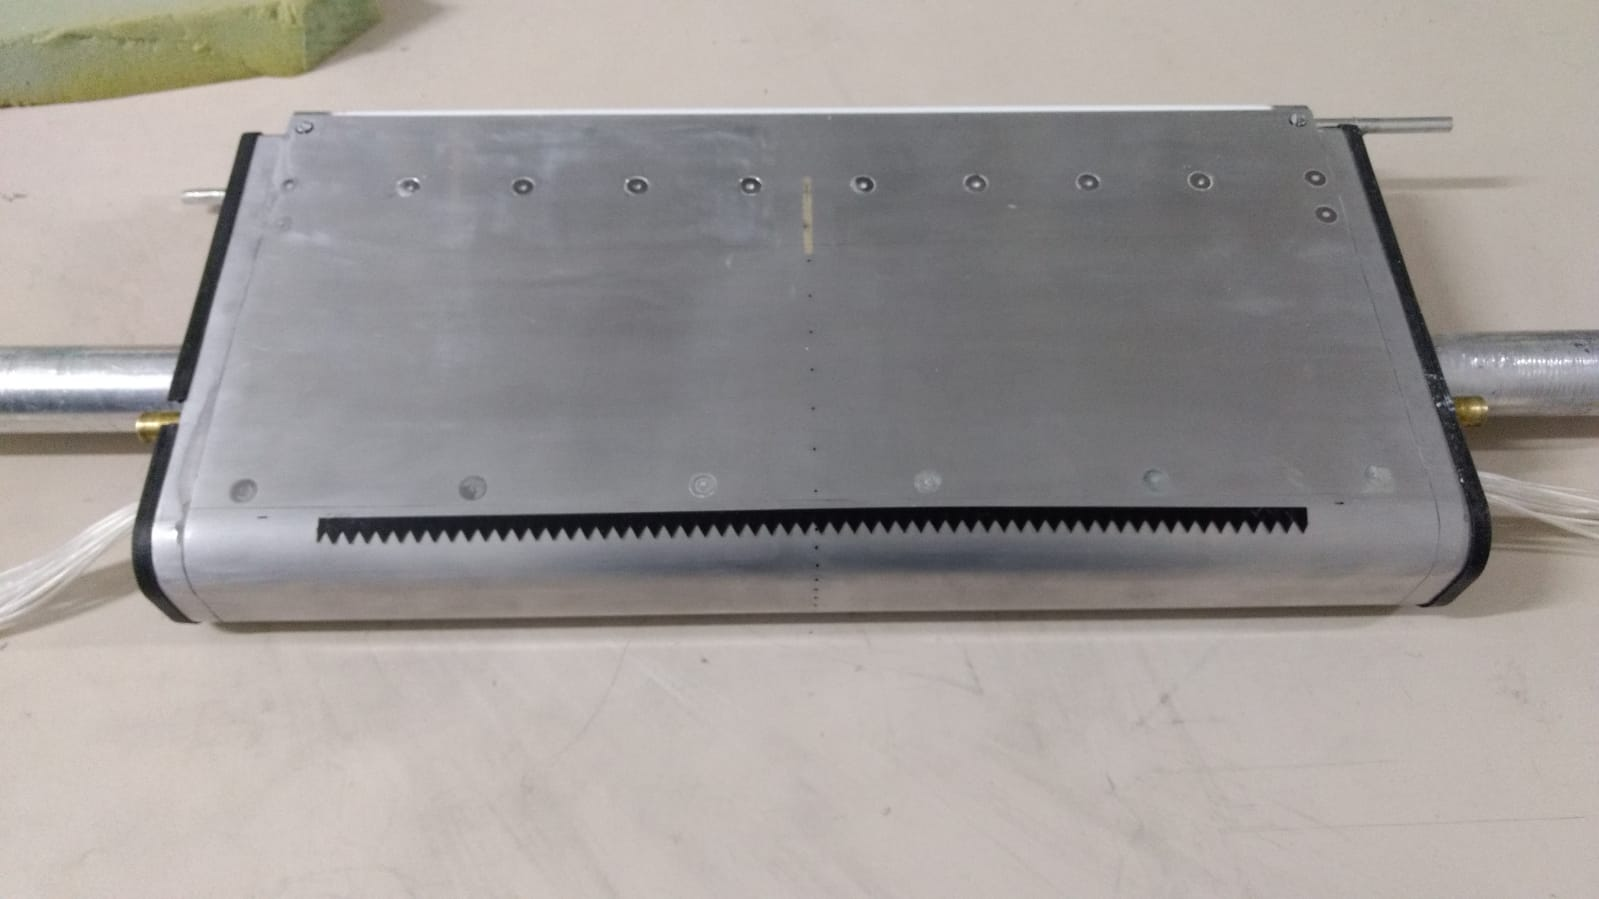
\includegraphics[width=0.55\textwidth]{DModell1.jpg}
%	\caption{Vorderansicht des Versuchsmodells mit Zackenband an Ober- und Unterseite.}
%	\label{fig:DModell1}
%\end{figure}
Wie in \abb{fig:DModell2} ersichtlich ist, sind an der R"uckseite des Stumpfk"orpers an Ober- und Unterseite des Modells jeweils 10 Schrauben montiert. Diese dienen der Einstellung des Ausblasespaltes. Das genaue Verfahren zur Einstellung des Spaltes wird in Abschnitt \ref{sec:Versuchsvorbereitung} erl"autert.


\begin{figure}[h]
	\centering
	\begin{subfigure}[c]{0.49\textwidth}		
		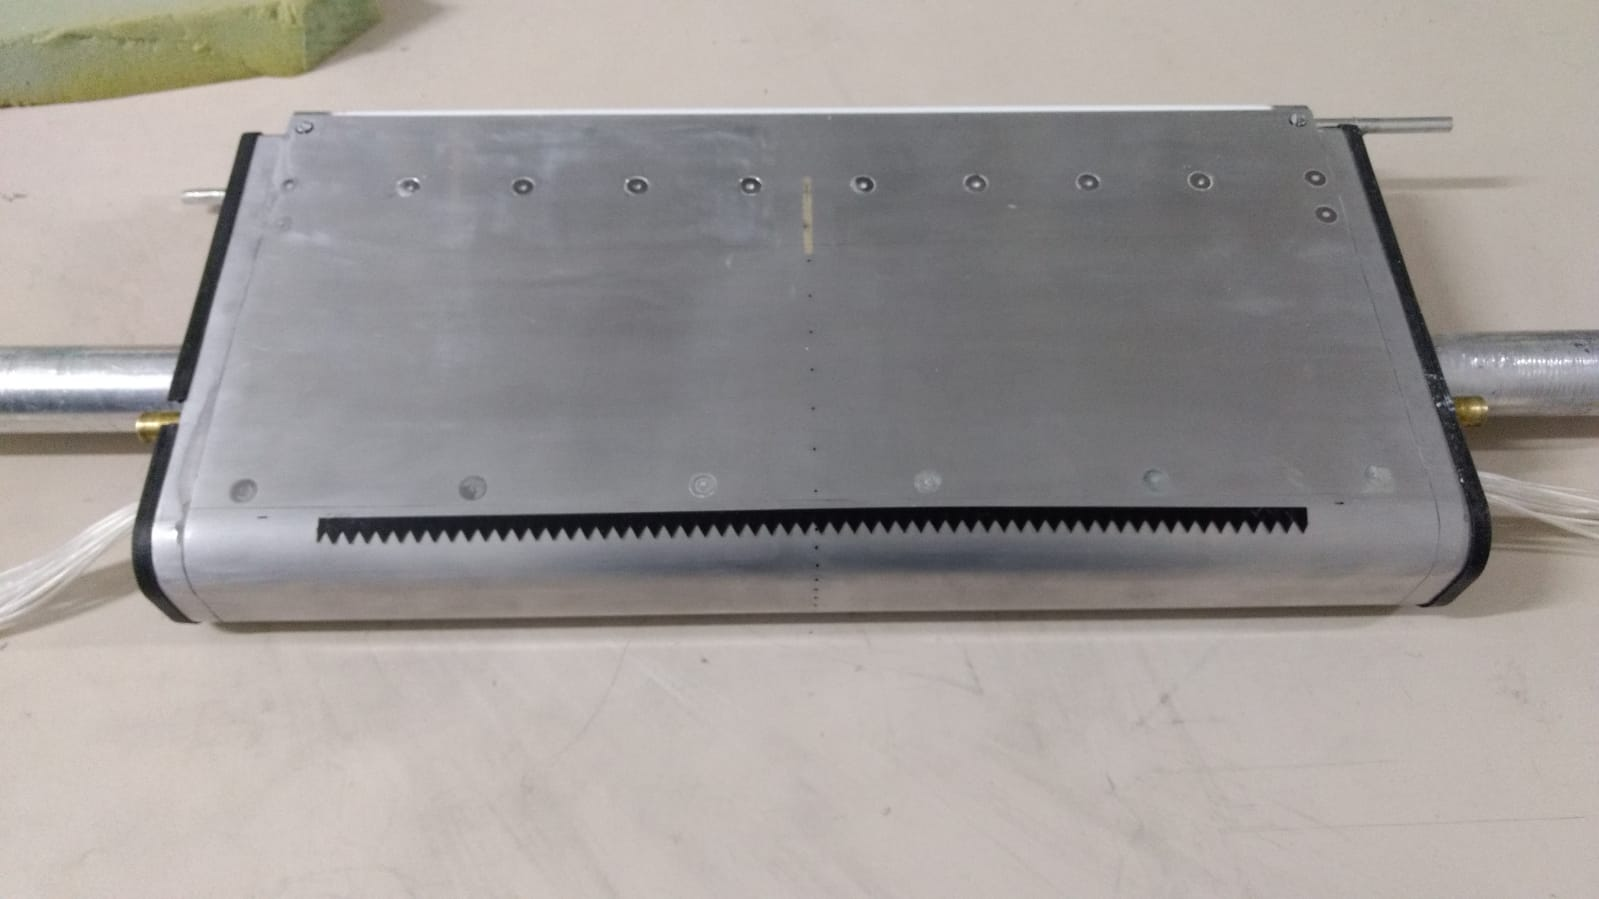
\includegraphics[width=1\textwidth]{DModell1.jpg}
		\subcaption{Vorderansicht mit Zackenband an Ober- und Unterseite.}
		\label{fig:DModell1}
	\end{subfigure}
	\begin{subfigure}[c]{0.49\textwidth}
		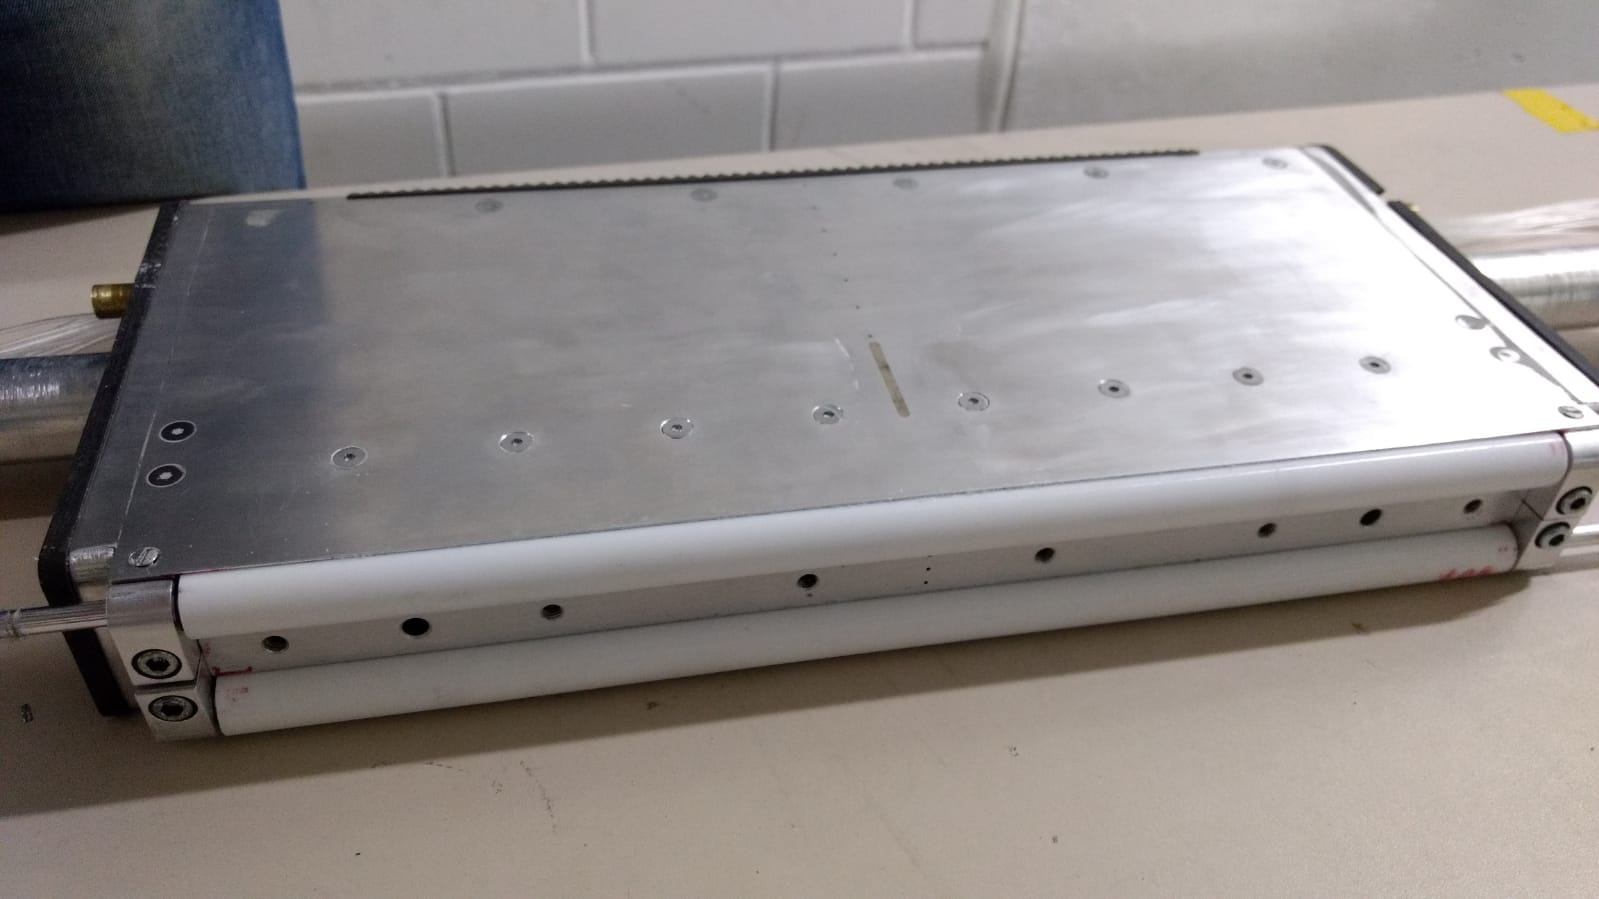
\includegraphics[width=1\textwidth]{DModell2.jpg}
		\subcaption{R"uckansicht mit eingebauten Tefolnwalzen.}
		\label{fig:DModell2}
	\end{subfigure}
	\caption{Ansicht des Versuchsmodells}
	\label{fig:DModell}
\end{figure}


%\begin{figure}[h]
%	\centering
%	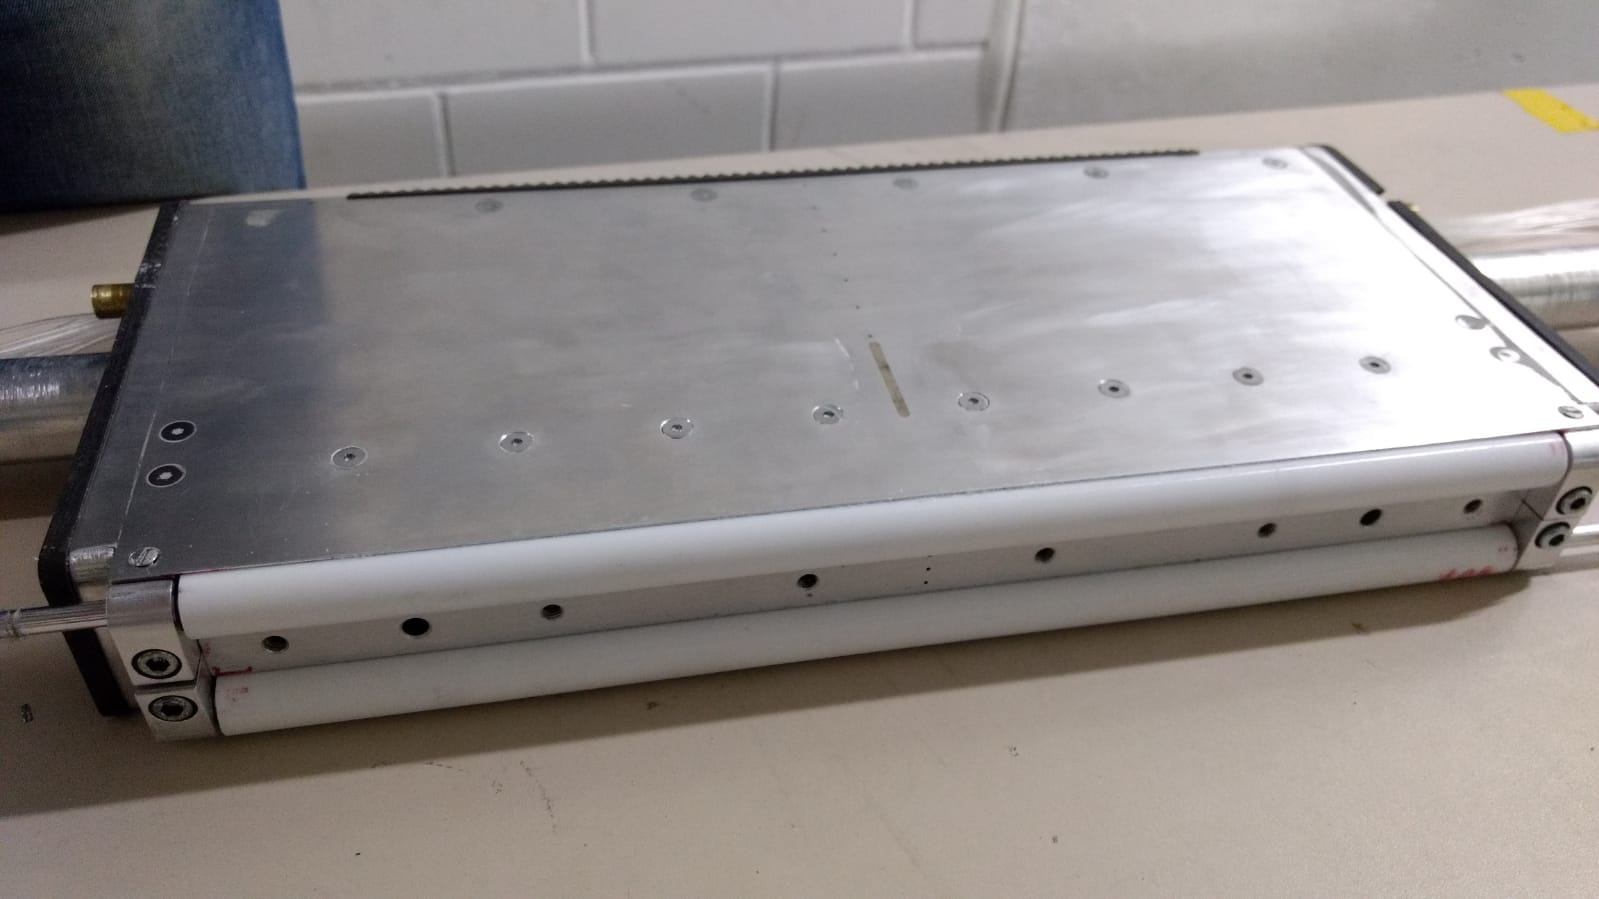
\includegraphics[width=0.55\textwidth]{DModell2.jpg}
%	\caption{R"uckansicht des Versuchsmodells mit eingebauten Tefolnwalzen.}
%	\label{fig:DModell2}
%\end{figure}

\clearpage
%%%%%%%%%%%%%%%%%%%%%%%%ENDE Modellbeschreibung Tim%%%%%%%%%%%%%%%%%%%%%%%%%%%%%



%%%%%%%%%%%%%%%%%%%%%%Kebria%%%%%%%%%%%%%%%%%%%%%%%%%%%%%%%%%%%%%

\section{Windkanalbeschreibung (KK)}
F"ur die experimentellen Untersuchungen steht der "Leiser Niedergeschwindigkeitskanal Braunschweig" (LNB) vom Institut f"ur Str"omungsmechanik der Technischen  Universit"at Braunschweig zur Verf"ugung.\\
Nach Eifel-Bauart erbaut, ist der LNB an beiden Enden offen und wird durch die Umgebungsluft im Raum versorgt. (\abb{fig:windkanal}).
Durch eine besondere Art der Polsterung bzw. Schalld"ampfer und einen
ger"auscharmen Elektroantrieb, ist dieser Windkanal f"ur einen m"oglichst leisen Betrieb konstruiert worden.
Testk"orper, die f"ur die Untersuchung eine maximale Anstr"omgeschwindigkeit von \SI{20}{\meter/\second} ben"otigen und die passende Gr"o\ss{}e haben, sind f"ur Versuche in diesem Windkanal geeignet.
\begin{figure}[h]
	\centering
	\begin{subfigure}[c]{0.6\textwidth}		
		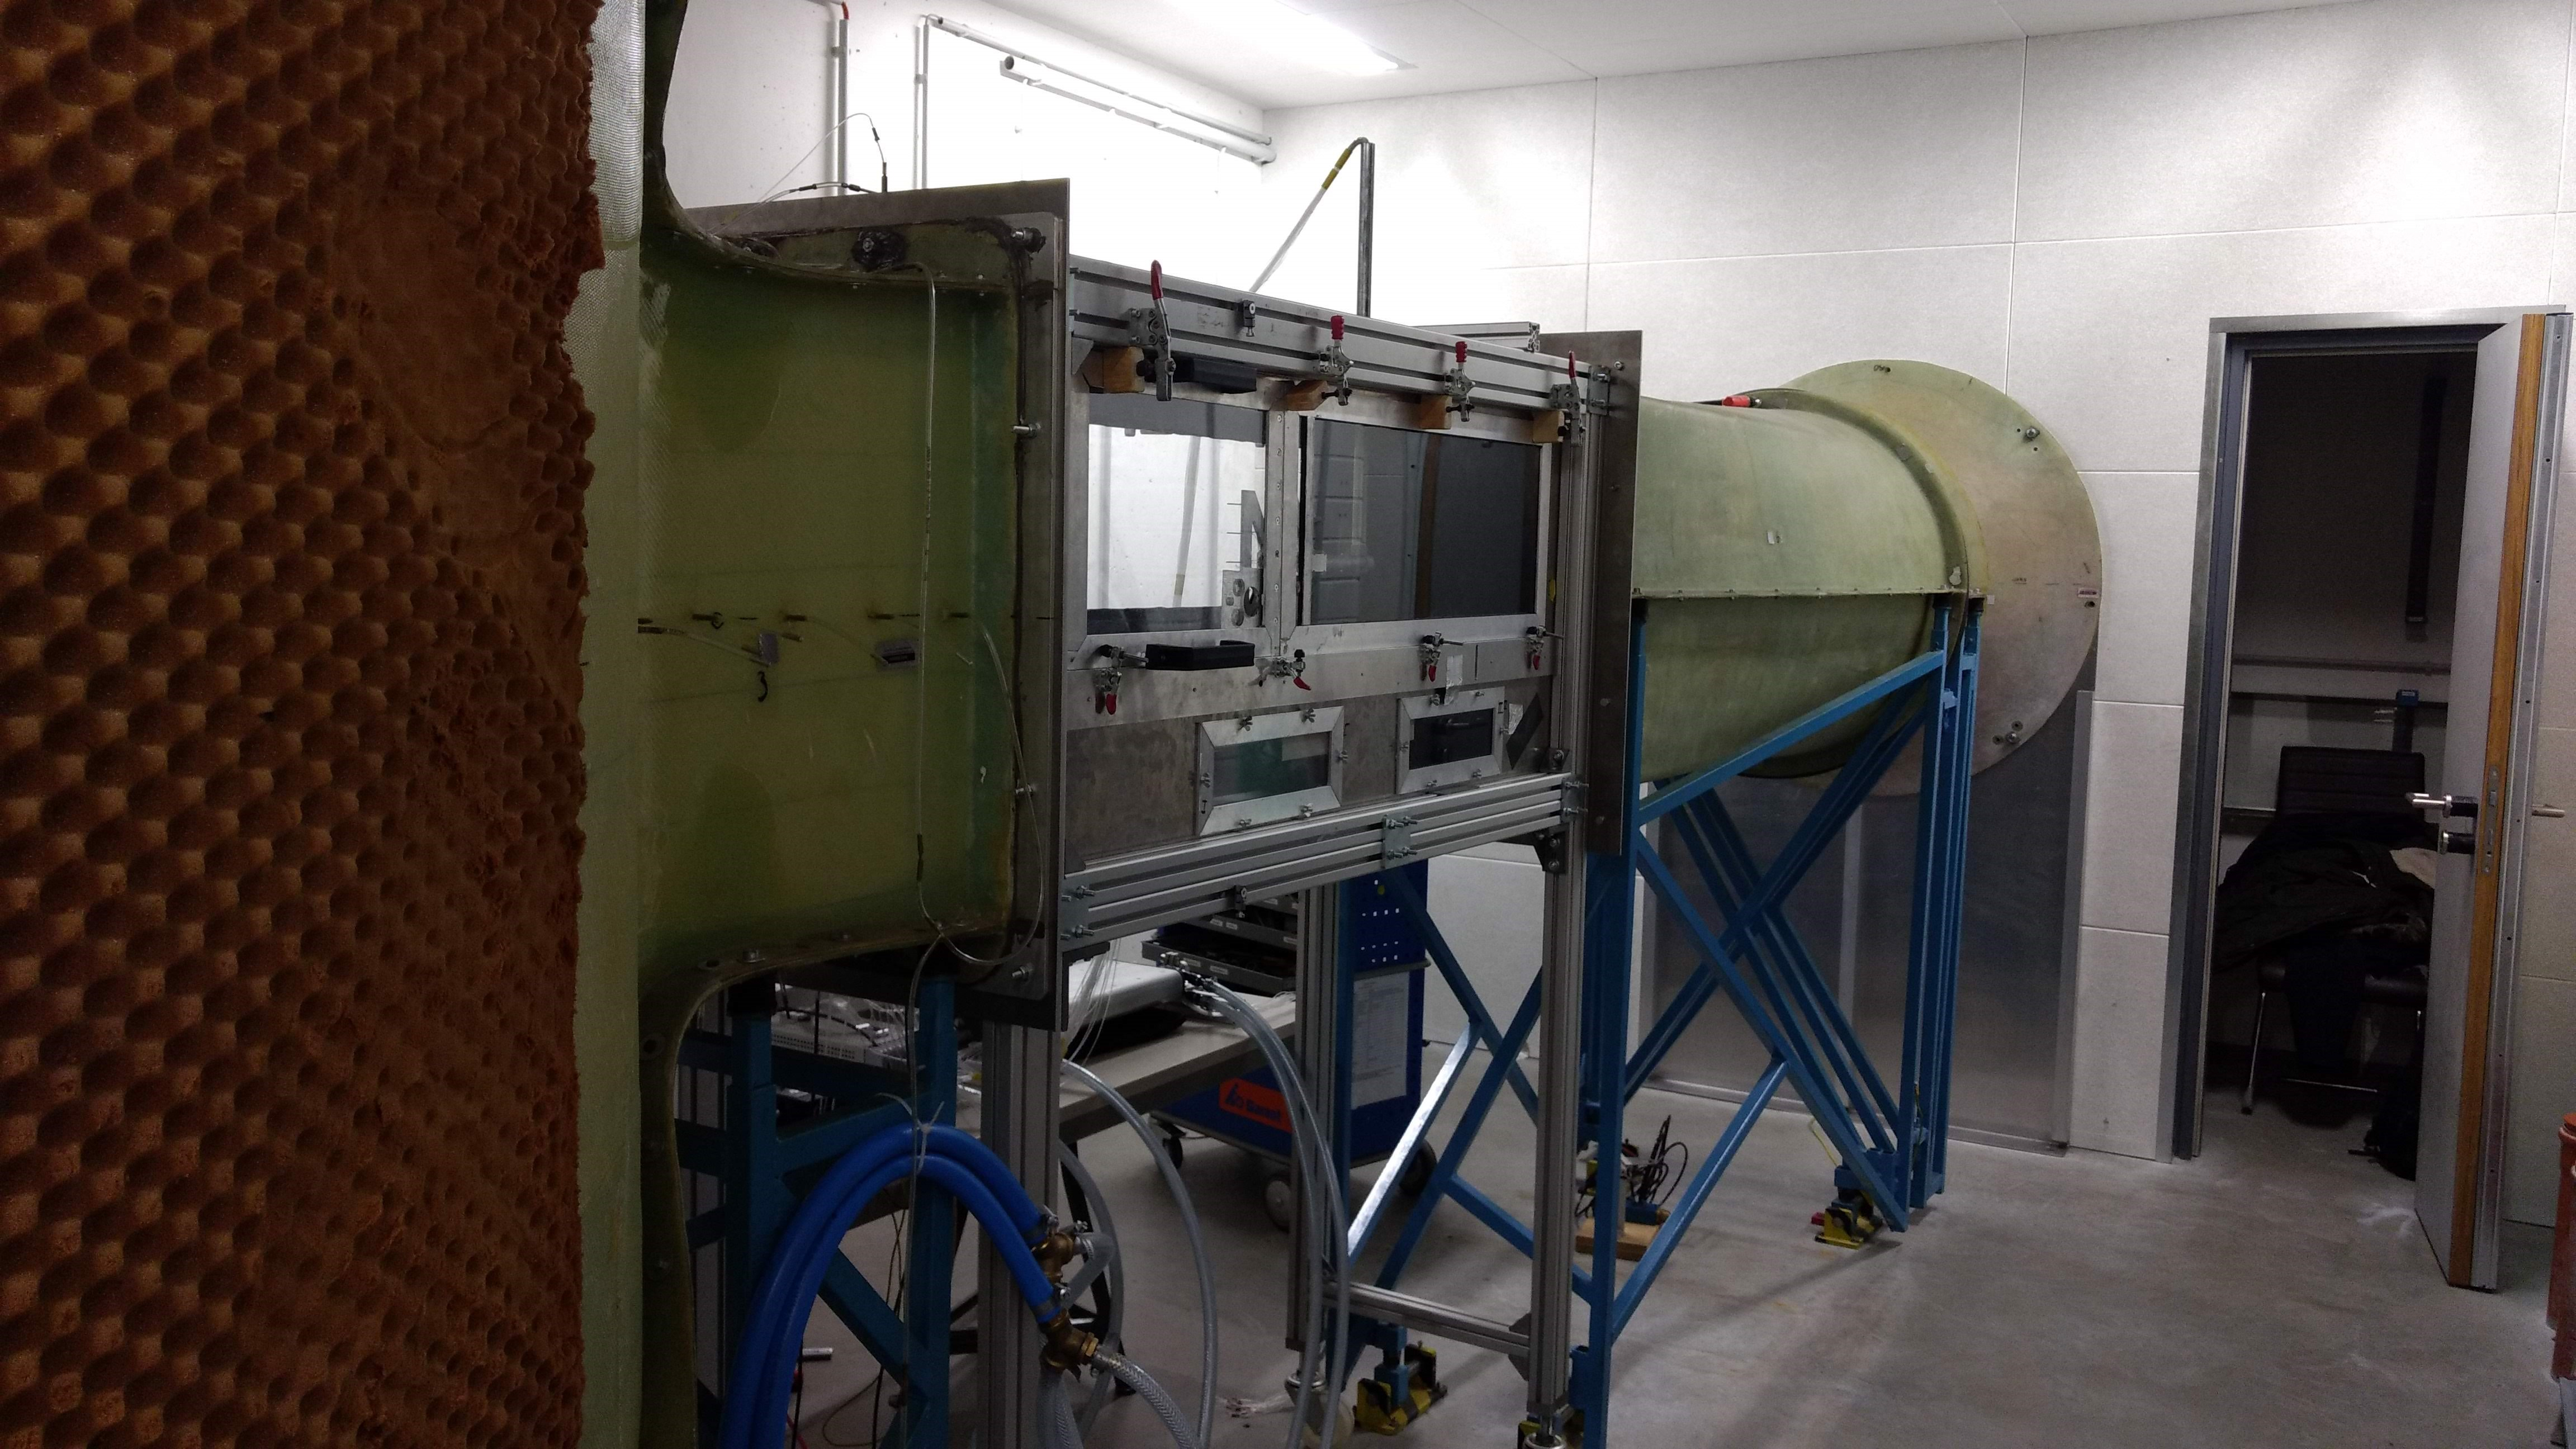
\includegraphics[width=1\textwidth]{windkanal1.jpg}
	\end{subfigure}
	\begin{subfigure}[c]{0.6\textwidth}
		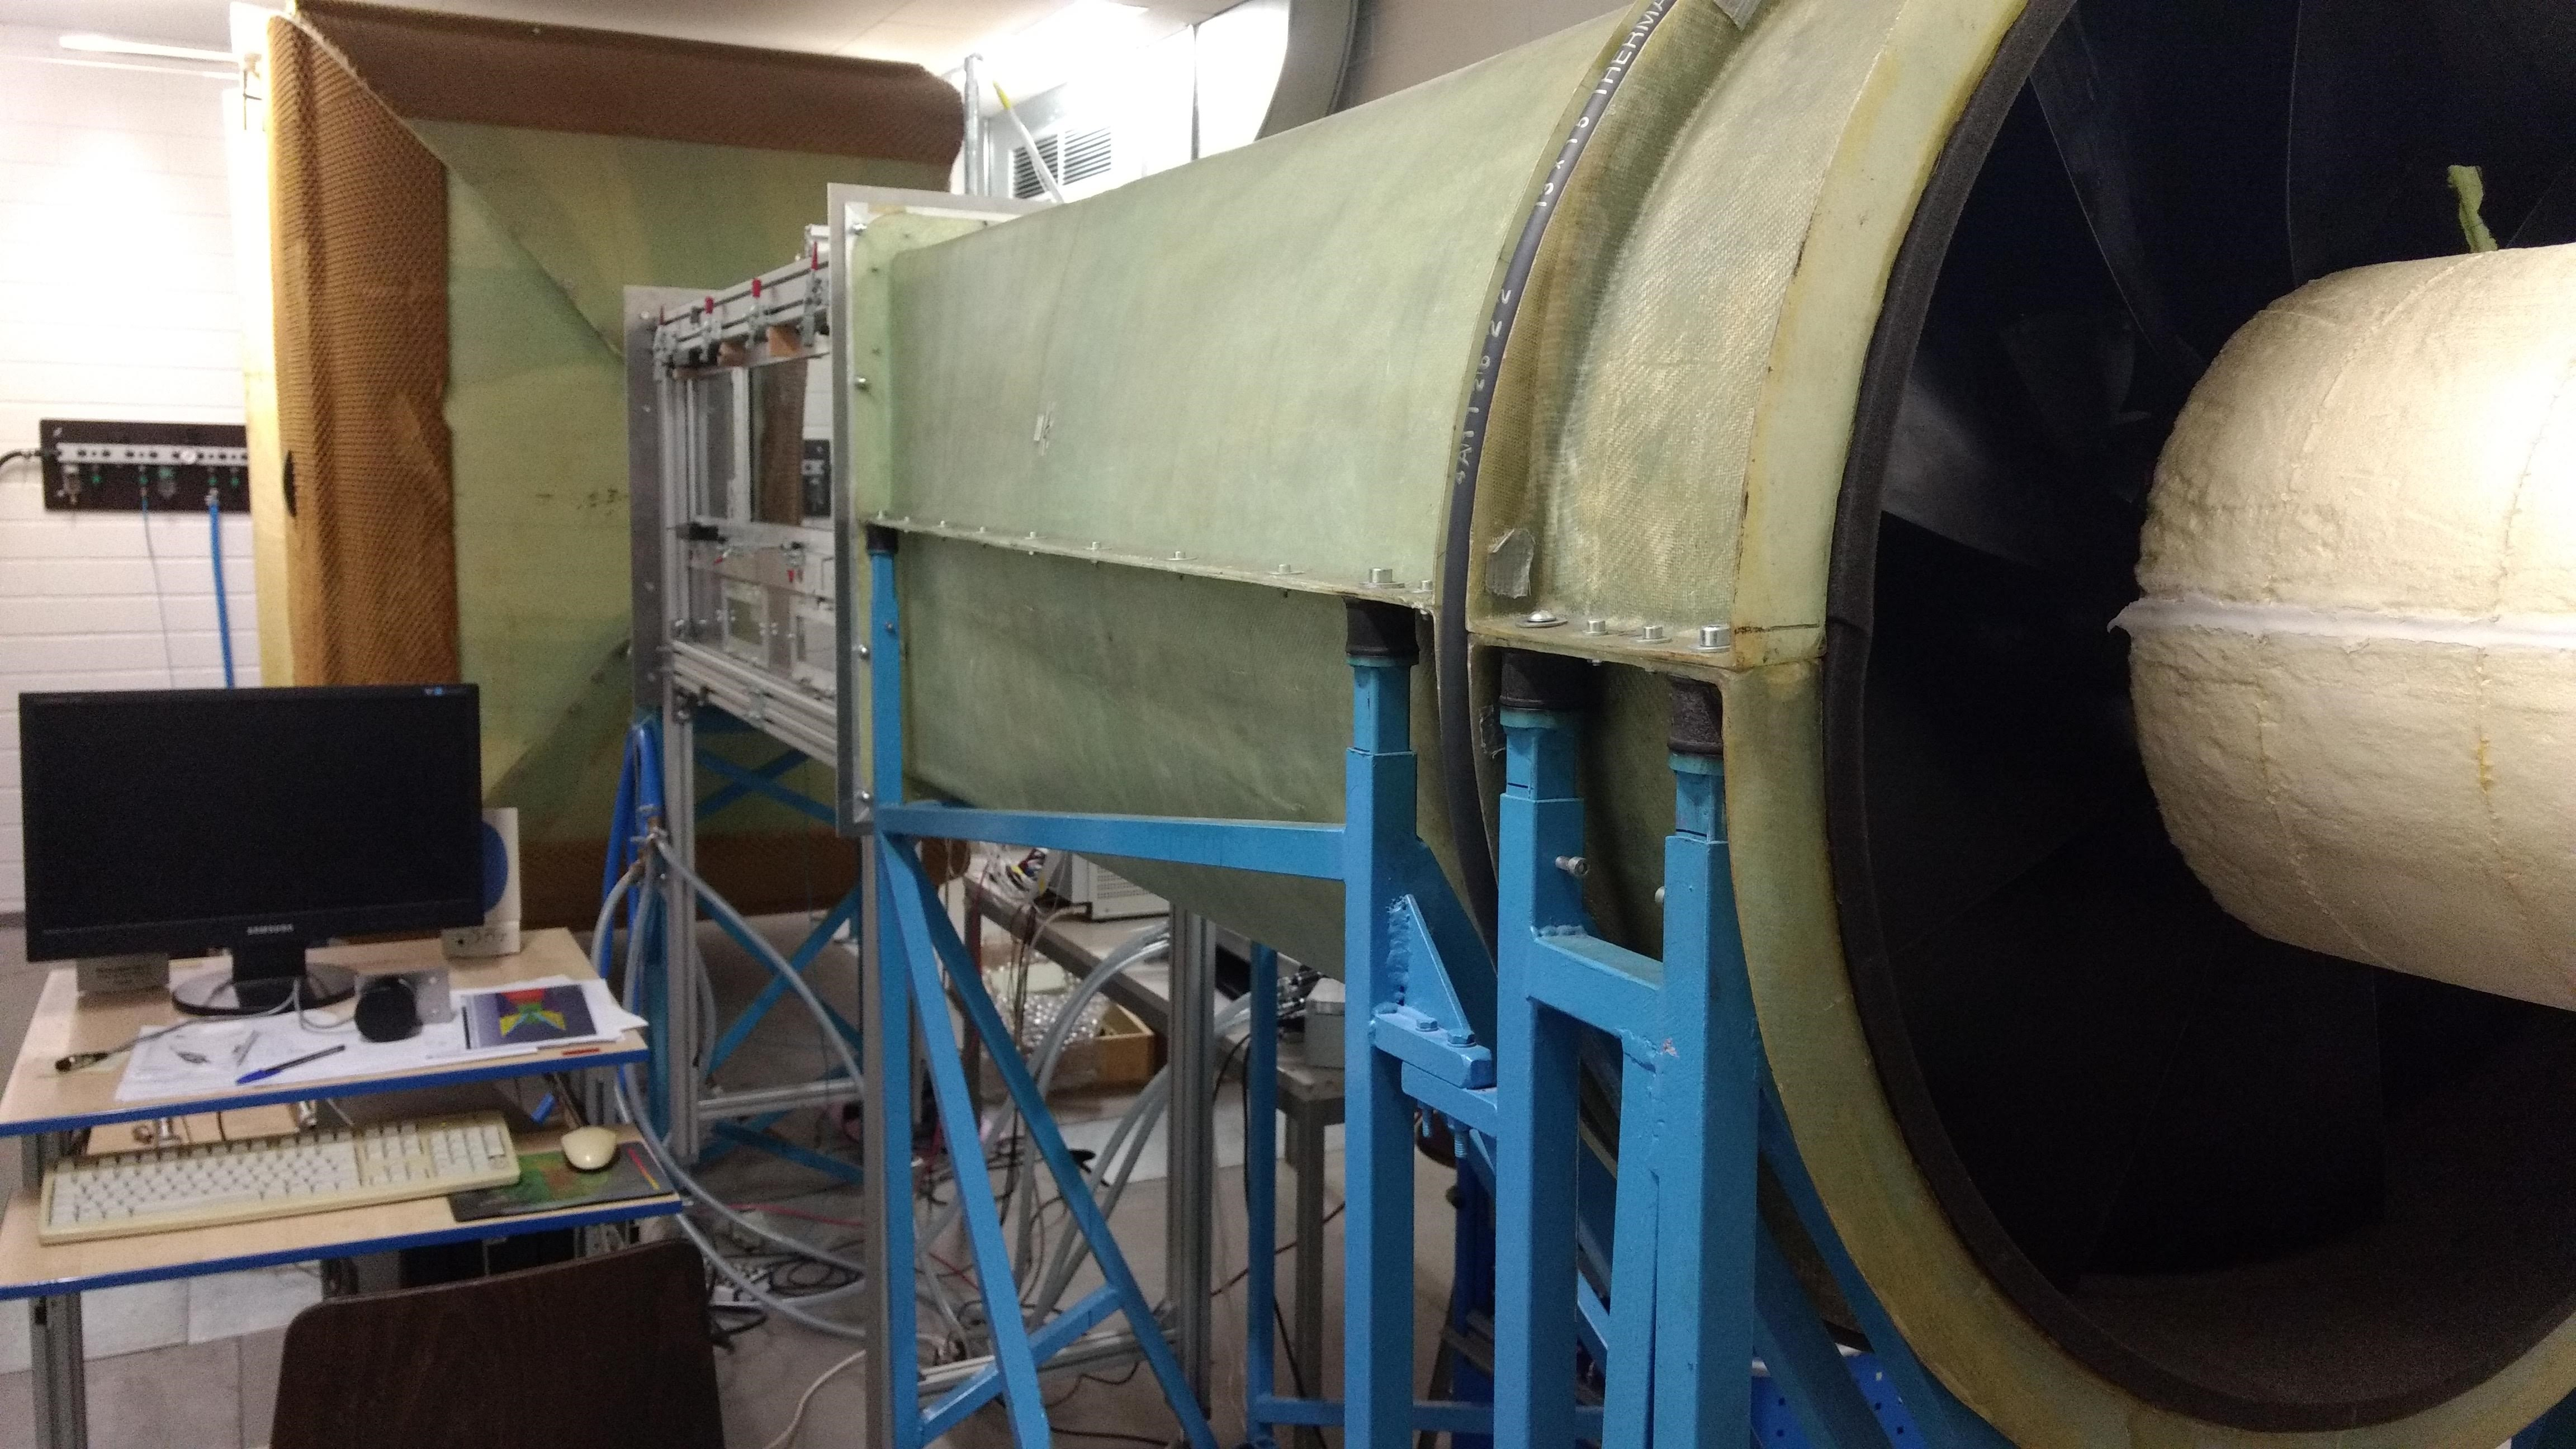
\includegraphics[width=1\textwidth]{windkanal2.jpg}
	\end{subfigure}
	\caption{LNB-ISM TU Braunschweig}
	\label{fig:windkanal}
\end{figure}\\


%\section{Messtechnik (KK)}
%Nicht nur bei der Versuchsvorbereitung, sondern auch w"ahrend des Versuchs werden Messger"ate und Einrichtungen ben"otigt, ohne die eine sinnvolle Untersuchung und rechnerische Ermittlungen der Versuchsparameter nicht m"oglich ist.
%
%Hier wird auf die f"ur den Versuch eingesetzten Messmittel und deren Funktionsweisen eingegangen.
%
%\subsection{Messuhr}
%Die Messuhr wird f"ur die Messung der L"angendifferenzen oder auch L"angen eingesetzt. Mit einer "ublichen Genauigkeit von \SI{10}{\micro\meter} und einem Messbereich von 5 bis \SI{60}{\milli\meter} eignen sich die Messuhren f"ur Parallelit"ats- und Ebenheitsmessungen.
%
%\subsection{Fischmaul-Sonde}
%Die Fischmaul-Sonde ist im Prinzip ein an der Spitze plattgedr"ucktes Pitot-Rohr. Sie eignet sich am besten f"ur Staudruckmessungen an bzw. in angestr"omten Spalten.
%
%\subsection{Statische Sonde}
%Die statische Sonde besitzt nur Bohrungen, die tangential zur Str"omung sind und deshalb nur für die Messung des statischen Drucks geeignet sind.
%Damit die Bohrungen m"oglichst keinen dynamischen Anteil messen, m"ussen sie sich weit genug entfernt von der Sondenspitze befinden, da in und nach diesem Bereich, die Str"omung umgelenkt wird und lokal nicht mehr tangential zu den Bohrungseintrittsfl"achen steht.
%
%\subsection{Prandtl-Sonde}
%Diese Sonde kombiniert die statische Sonde und das Pitot-Rohr.
%Die von der seitlichen Bohrungen gemessenen Dr"ucke laufen im inneren System gegen den an der Spitze gemessenen Staudruck.
%Somit wird der statische Druck vom Gesamtdruck abgezogen und der dynamische Druck erhalten. Durch weitere Rechnungen ist es m"oglich, mittels dynamischen Drucks die Anstr"omgeschwindigkeiten zu berechnen.
%
%\subsection{Drehzahlmesser}
%
%\subsection{PSI-Anlage}

\section{Versuchsvorbereitung}
\label{sec:Versuchsvorbereitung}
\subsection{Vorgehensweise (KK)}
Nicht nur bei der Versuchsvorbereitung, sondern auch w"ahrend des Versuchs werden Messger"ate und -einrichtungen ben"otigt, ohne die eine sinnvolle Untersuchung und rechnerische Ermittlungen der Versuchsparameter nicht m"oglich sind.\\
Vor einer Windkanaluntersuchung sollte man mit diesen Messmitteln vertraut sein und den Windkanal f"ur die Testanforderungen und die Eigenschaften des Testk"orpers vorbereiten.

In diesem Kapitel werden die vorbereitenden Prozeduren und der Umgang mit den daf"ur ben"otigten Messmitteln n"aher beschrieben.

Bei einem Windkanalversuch sollte eine m"oglichst hohe Sauberkeit des Testk"orpers und des Windkanals gew"ahrleistet werden. Kleine Fremdk"orper und Partikel am K"orper sowie den f"ur die Untersuchung wichtigen Bereichen die Str"omung und die zu erwartenden Effekte und Ph"anomene ungewollt beeinflussen k"onnen. Au\ss{}erdem k"onnen die Sonden und weitere Messger"ate verstopft oder besch"adigt werden.

Um den Druckverlauf am Ausblaseschlitz messen zu k"onnen, muss der Testk"orper m"oglichst parallel zu der beweglichen Achse der Druckmessonde befestigt sein. Bereits geringe Parallelit"atsabweichungen von weniger als 100\,$\mu$m auf die Testk"orperbreite von 390\,mm k"onnen zu fehlerhaften Messungen f"uhren. Deshalb wird die Parallelit"at mithilfe einer Messuhr eingestellt. Die Messuhr wird f"ur die Messung der L"angendifferenzen oder L"angen eingesetzt. Mit einer "ublichen Genauigkeit von 10\,$\mu$m und einem Messbereich von 5 bis 60\,mm eignen sich Messuhren f"ur Parallelit"ats- und Ebenheitsmessungen.

Der Totaldruck am Ausblaseschlitz wird mit einer Fischmaulsonde (s. \abb{fig:Fischmaulsonde}) gemessen. Die Fischmaulsonde ist ein an der Spitze plattgedr"ucktes Pitot-Rohr. Sie eignet sich am besten f"ur Staudruckmessungen an bzw. in angestr"omten Spalten. Ein "ublches Pitot-Rohr besitzt eine Messbohrung an der Spitze, die normal zur Str"omung steht. Somit werden sowohl der dynamische als auch der statische Druck zusammen aufgenommen. Dieser Druck wird auch als Staudruck bezeichnet und entspricht dem Gesamtdruck der Str"omung.

\begin{figure}[h]
	\centering
	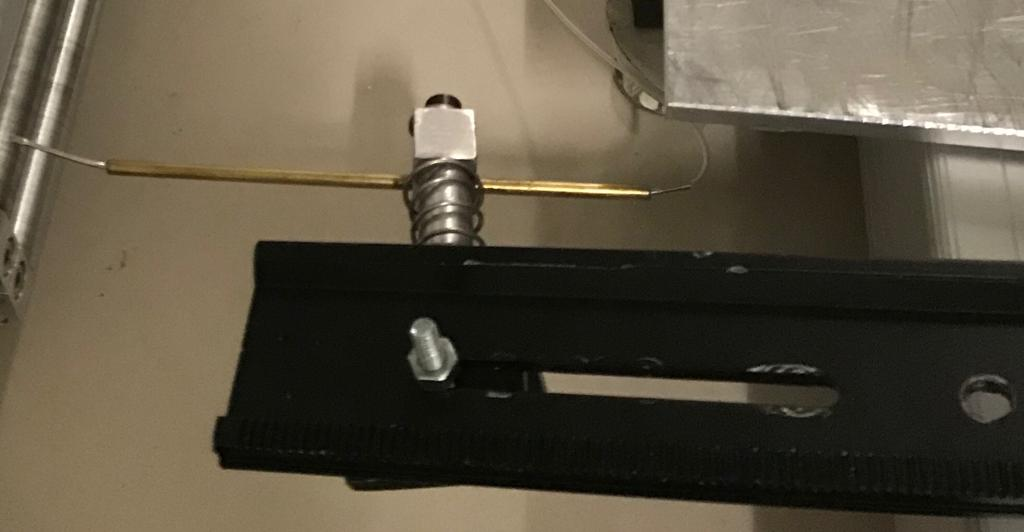
\includegraphics[width=0.6\textwidth]{Fischmaulsonde.jpg}
	\caption{Fischmaulsonde}
	\label{fig:Fischmaulsonde}
\end{figure}

Die Druckmesssonden - wie unter anderem die Fischmaulsonde - sind mittels d"unnen Schl"auchen mit einem oder mehreren Messmodulen verbunden, die mithilfe der piezoelektrischen Messanlage den Druck berechnen lassen. Hierbei wird der Umgebungsdruck als Referenz herangezogen.

Nachdem die Gleichm"a\ss{}igkeit des Druckverlaufs erzeugt wurde, k"onnen die Druckluftschl"auche, die f"ur die Ausblasung notwendig sind, angeschlossen und der Testk"orper eingebaut werden. Auf die Erzeugung des gleichm"a\ss{}igen Druckverlaufs wird noch genauer in \abschn{s:Gleichf"ormigkeitsmessungen} eingegangen. Sie ist f"ur die Erm"oglichung der Annahme einer zweidimensionalen Str"omung notwendig.

Da bei diesem Experiment ein symmetrischer Testk"orper mit gegenl"aufigen Wellen untersucht wird, muss dieser auch symmetrisch eingebaut werden, sodass die Druckverteilung auf der Ober- und Unterseite gleich ist.

Der Druckverlauf und die Nachlaufdelle hinter dem K"orper wird mit einem Druckmessrechen gemessen.\\
Der Rechen im Einsatz hinter dem Modell ist in \abb{fig:Druckmessrechen} zu sehen.
\begin{figure}[h]
	\centering
	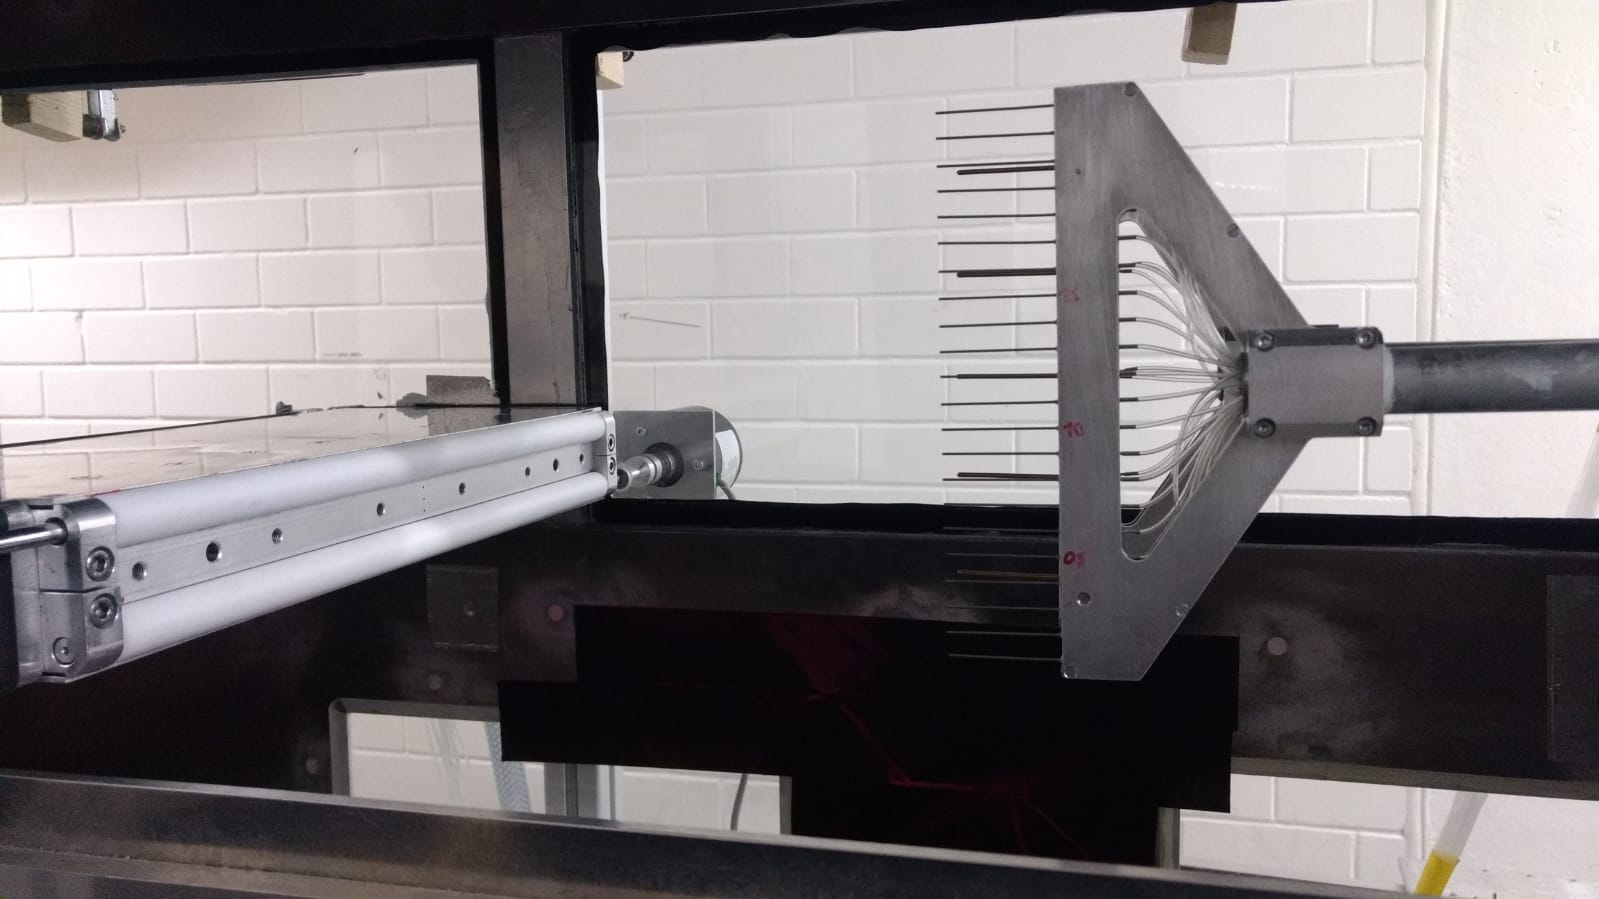
\includegraphics[width=0.6\textwidth]{Druckmessrechen_mitModell.jpg}
	\caption{Druckmessrechen w"ahrend des Versuchs}
	\label{fig:Druckmessrechen}
\end{figure}
Dieser muss gen"ugend Abstand von der Hinterkante des Testk"orpers haben, damit die Verwirbelungen im Totwassergebiet keinen Messfehler verursachen.\\
Der im Versuch eingesetzte Rechen ist mit 22 Pitot-Sonden und f"unf Prandtl-Sonden ausgestattet.
%Letztere werden vornehmlich dazu gebraucht, den statischen Druck zu messen. Sie fungieren somit als statische Sonden.\\

Die Prandtl-Sonden werden in diesem Versuch jedoch als statische Sonden eingesetzt.

Eine statische Sonde besitzt nur Bohrungen, die tangential zur Str"omung angebracht sind und deshalb nur f"ur die Messung des statischen Drucks geeignet sind.
Damit die Bohrungen m"oglichst keinen dynamischen Druckanteil messen, m"ussen sie sich weit genug entfernt von der Sondenspitze befinden, da in und nach diesem Bereich die Str"omung umgelenkt wird und lokal nicht mehr tangential zu den Bohrungsfl"achen steht.

Eine Prandtl-Sonde kombiniert die statische Sonde und das Pitot-Rohr.\\
Die von der seitlichen Bohrungen gemessenen Dr"ucke laufen im inneren System gegen den an der Spitze gemessenen Staudruck.\\
Somit wird der statische Druck vom Gesamtdruck abgezogen und der dynamische Druck bleibt erhalten.
%Durch weitere Rechnungen ist es m"oglich, mittels dynamischen Drucks die Anstr"omgeschwindigkeit zu berechnen.

Die Anzahl der Pitot-Sonden sind deutlich h"oher als die der eingesetzten Prandtl-Sonden, da sich die Prandtl-Sonden wie oben beschrieben "uber seitliche Messbohrungen tangential zur Str"omung verf"ugen. Die Umstr"omung einer Sonde erzeugt einen dynamischen Anteil quer zur Hauptstr"omung. Dieser muss einen m"oglichst gro\ss{}en Abstand von der seitlichen Messbohrung der h"oher liegenden Sonde haben, um die Messfehler gering zu halten.

Da die Pitot-Sonden sich nicht in dieser Form einschr"anken bzw. st"oren lassen, kann - zugute einer hohen Aufl"osung - eine gr"o\ss{}ere Anzahl von dieser Art Sonde eingesetzt werden.

Wie in diesem Versuch, kann es passieren, dass der Druckrechen nicht ausreichend gro\ss{} ist, um den kompletten Nachlauf abzudecken.\\
Aus diesem Grund wird der Rechen asymmetrisch eingebaut, um Dr"ucke am Nachlaufrand messen zu k"onnen. Da der Testk"orper symmetrisch gefertigt und eingebaut ist, wird ein symmetrischer Druckverlauf erwartet. Somit k"onnen die vom Rechen nicht abgedeckten Druckmesspunkte von der gegen"uberliegenden gedeckten Seite "ubernommen werden.

Nach dem Einbau des Testk"orpers und dem Einstellen des Rechens k"onnen die Motoren "uber die Sicherheitskupplungen an den Wellen befestigt werden.

%Ende KEBRIA
%------------------------------------------------------------------------------------------------------------------------------------------------------------------------------------------
%Anfang AMIRIMAN

\subsection{Gleichf"ormigkeitsmessungen an der Ausblasung (AK)}
\label{s:Gleichf"ormigkeitsmessungen}
Um die sp"atere Zuordnung zu erleichtern bekommen die verschiedenen Konfigurationen des Modells zun"achst Namen, die in \tab{tab:zuordnung} zu sehen sind.

\begin{table}[h]
	\centering
	\begin{tabular}{ll}
		\toprule
		Beschreibung & Name\\
		\midrule
		Modell mit eingebauten glatten Wellen & Basiskonfiguration\\
		Modell mit eingebauten ovalen Wellen (33\,\% duty cycle) & Konfiguration 33\\
		Modell mit eingebauten ovalen Wellen (50\,\% duty cycle) & Konfiguration 50\\
		\bottomrule
	\end{tabular}
	\caption{Bezeichnungen der verschiedenen Konfigurationen}
	\label{tab:zuordnung}
\end{table}
Konfiguration 33 kann wegen zu gro\ss{}er Fertigungsungenauigkeiten nicht bei den Messungen ber"ucksichtigt werden.

Die Messung der Druckgleichf"ormigkeit wird einmal mit den glatten und einmal mit den ovalen Wellen mit 50\,\$ duty cycle durchgef"uhrt. Die Basis Konfiguration bei der Vermessung der Gleichf"ormigkeit ist in  \abb{fig:Modell_bei_Gleichf"ormigkeitsmessungen} zu sehen.

\begin{figure}[h]
	\centering
	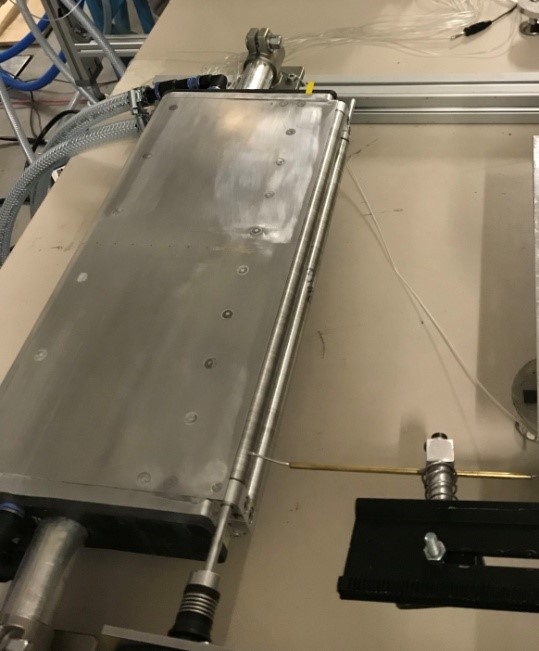
\includegraphics[width=0.4\textwidth]{Modell_bei_Gleichfoermigkeitsmessungen_glatt.jpg}
	\caption{Gleichf"ormigkeitsmessungen am Modell mit eingebauten glatten Walten}
	\label{fig:Modell_bei_Gleichf"ormigkeitsmessungen}
\end{figure}

Durch vier Schl"auche, die an einem Kompressor mit 8 bar Druck angeschlossen sind, wird die Druckluft den beiden Plenen zugef"uhrt. Damit die Str"omung gleichf"ormig bleibt, sind die beiden Plenen gro\ss{} ausgelegt. 

Bei der Gleichf"ormigkeitsvermessung, muss beachtet werden, dass der Druck im ausgeblasenen Luftstrahl 1000\,Pa nicht "uberschreitet, damit die Fischmaulsonde nicht besch"adigt wird.\\
Die Spalth"ohe der beiden Ausblaseschlitze sollte "uber die gesamte Spannweite 0.3\,mm betragen. Dadurch wird sichergestellt, dass es keine spannweitigen Unterschiede in der Ausblasung und Str"omung gibt.
Fertigungsbedingt weichen die Spalth"ohen an den Modellr"andern aber von den geforderten 0,3\,mm ab. Zudem h"angen die glatten Wellen in der Mitte um etwa 0,04\,mm durch~\cite{Bilges.2018}. Aus diesem Grund wurde die Druckmessung mit langsam rotierenden Wellen durchgef"uhrt, was zu genaueren gemessenen Druckverteilungen f"uhrt.

Das Modell verf"ugt an Ober- und Unterseite "uber jeweils 8 Einstellschrauben, mit denen die Spalte lokal geschlossen und ge"offnet werden k"onnen. Des Weiteren 
Durch Vergleich mit F"uhlerlehren werden an den glatten Wellen jeweils Spalth"ohen eingestellt, die "uber die Spannweite zwischen 0,25\,mm und 0,3\,mm liegen.

W"ahrend der Messungen, werden au\ss{}erdem beide Plenumsinnendr"ucke dauerhaft kontrolliert und somit sichergestellt, dass die Ausblasung "uber die Spalte optimal und ohne starke Unterschiede zwischen Unter- und Oberseite abl"auft.
Bei einem mittleren Plenumsdruck von 500\,Pa unterscheiden sich die Dr"ucke um maximal 5\,\%. Diese Abweichung ist auf die innere Struktur des Modells zur"uckzuf"uhren.

F"ur die Druckmessungen wird das Modell mit den glatten Wellen parallel zu einer Traverse ausgerichtet, auf der die Fischmaulsonde angebracht ist. Die Sonde l"asst sich auf der Traverse manuell spannweitig verfahren. 

\abb{fig:Druckverteilung_glatt_oben} zeigt die Druckverteilung der oberen glatten Walze bei niedriger Drehzahl "uber der spannweitigen Koordinate in Prozent. Es ist deutlich zu erkennen, dass die Punkte in Randn"ahe deutlich st"arker vom Mittelwert abweichen, als die "ubrigen Werte. Diese Abweichungen sind durch die nicht beeinflussbaren, fertigungsbedingten Unterschiede des Spalts in Randn"ahe zu erkl"aren.
Jeweils 10\,\% vom linken Rand und rechten Rand werden infolgedessen bei der Beurteilung der Gleichf"ormigkeit vernachl"assigt.

\begin{figure}[h]
	\centering
	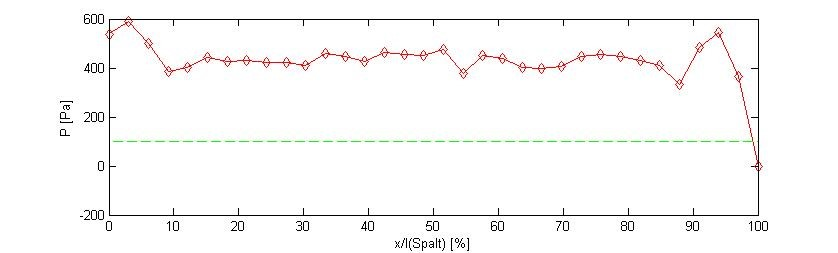
\includegraphics[width=0.85\textwidth]{GFM_Druckverteilung_glatt_oben.jpg}
	\caption{Druckverteilung der oberen glatten Welle in Pa "uber der spannweitigen Position in \%}
	\label{fig:Druckverteilung_glatt_oben}
\end{figure}

Damit ergeben sich f"ur die Druckverteilung an der oberen, glatten Welle ein Mittelwert von 428,8\,Pa und eine Standardabweichung von 7,5\,\% bei einer zul"assigen Standardabweichung von 10\,\%, die sich aus vorherigen Arbeiten als angemessen erwiesen hat.

In \abb{fig:Druckverteilung_glatt_unten} ist die Druckverteilung der unteren glatten Welle zu sehen.
Auch bei dem unteren Spalt werden die R"ander bei der Berechnung der Kennwerte f"ur die Gleichm"a\ss{}igkeit vernachl"assigt.
Bei einem Mittelwert von 457,8\,Pa wird eine Standardabweichung von 7\,\% ermittelt.

\begin{figure}[h]
	\centering
	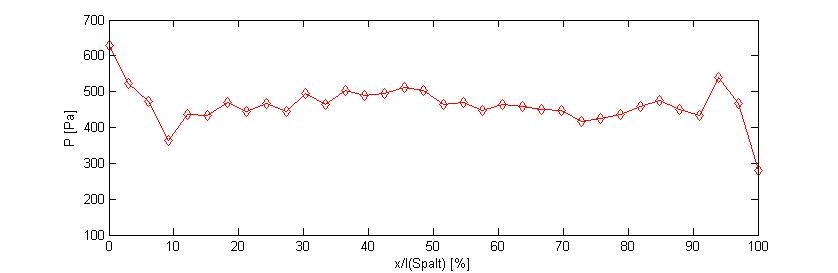
\includegraphics[width=0.85\textwidth]{GFM_Druckverteilung_glatt_unten.jpg}
	\caption{Druckverteilung der unteren glatten Welle in Pa "uber der spannweitigen Position in \%}
	\label{fig:Druckverteilung_glatt_unten}
\end{figure}

Dieselbe Art von Messung muss bei Anwendung auf die ovalen Wellen modifiziert werden, da die Spalth"ohe bei einer Umdrehung schwankt.
Um trotz variabler Spalth"ohe vergleichbare Daten zu erhalten, werden bei dieser Konfiguration die Messungen bei zwei definierten Wellenstellungen relativ zur Modellkante durchgef"uhrt.

In der ersten Stellung sind die Spalte komplett geschlossen, denn der gr"o\ss{}te Wellendurchmesser befindet sich im Spaltquerschnitt.
Die Spalte werden "uber die Schrauben so eingestellt, dass sich spannweitige Druckverteilungen ergeben, bei der $p$ "uberall 0\,Pa oder nahezu null wird.

\abb{fig:Druckverteilung_oval_geschl} zeigt die Druckverteilungen aus den entsprechenden Messungen an Ober- und Unterseite.

\begin{figure}[h]
	\centering
	\begin{subfigure}[c]{0.85\textwidth}		
		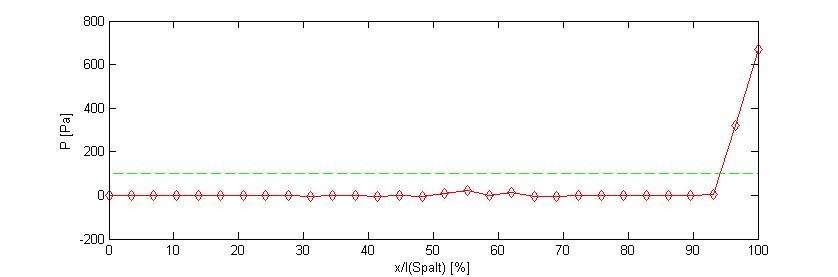
\includegraphics[width=1\textwidth]{GFM_Druckverteilung_oval_oben_geschl.jpg}
	\end{subfigure}
	\begin{subfigure}[c]{0.85\textwidth}
		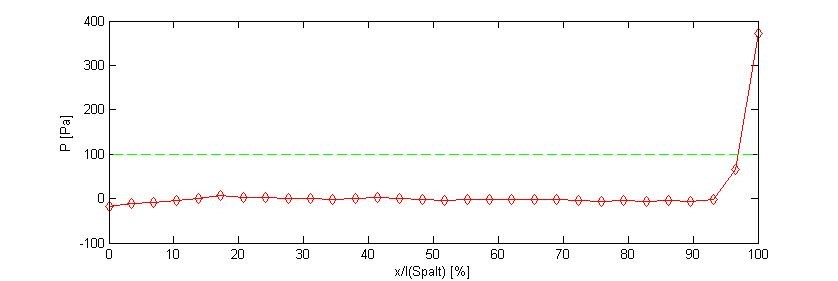
\includegraphics[width=1\textwidth]{GFM_Druckverteilung_oval_unten_geschl.jpg}
	\end{subfigure}
	\caption{Druckverteilungen der oberen (oben) und unteren (unten) ovalen Wellen in Stellung mit geschlossenem Spalt}
	\label{fig:Druckverteilung_oval_geschl}
\end{figure}

Es ist zu erkennen, dass bis auf die Randbereiche, glecihm"a\ss{}ige Druckverteilungen um 0\,Pa gegeben sind.

Der n"achste Schritt der Einstellung besteht darin, die Wellen in einer Position zu platzieren, in der die Spalte maximal ge"offnet sind. Auch bei den ovalen Wellen wurde die Spalth"ohe bei dieser Position zwischen 0,25\,mm und 0,3\,mm eingestellt. Diese Einstellung ist allerdings dadurch begrenzt, dass in der Stellung mit geschlossenem Spalt trotzdem noch die Druckverteilung nahe 0\,Pa sichergestellt werden muss. \abb{fig:Druckverteilung_oval_geschl} zeigt die finalen Verteilungen, der "Uberpr"ufungsmessung f"ur Position 1 nach Einstellung des Spalts in der zweiten Position.  
In \abb{fig:Druckverteilung_oval_offen} sind die spannweitigen Dr"ucke f"ur die ovalen Wellen in Position 2 zu sehen.

\begin{figure}[h]
	\centering
	\begin{subfigure}[c]{0.85\textwidth}		
		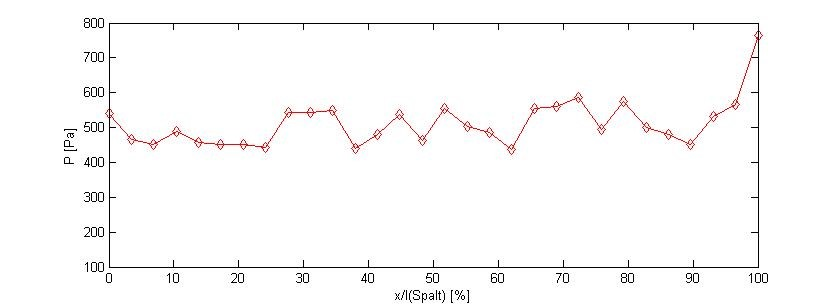
\includegraphics[width=1\textwidth]{GFM_Druckverteilung_oval_oben_offen.jpg}
	\end{subfigure}
	\begin{subfigure}[c]{0.85\textwidth}
		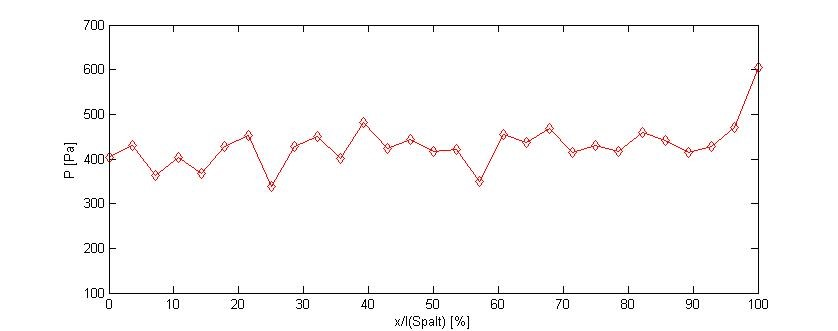
\includegraphics[width=1\textwidth]{GFM_Druckverteilung_oval_unten_offen.jpg}
	\end{subfigure}
	\caption{Druckverteilungen der oberen (oben) und unteren (unten) ovalen Wellen in Stellung mit maximal ge"offnetem Spalt}
	\label{fig:Druckverteilung_oval_offen}
\end{figure}

F"ur die Spalte mit ovalen Wellen ergeben sich die Standardabweichungen 9,5\,\% (oben) und 8,3\,\%(unten).

Die Standardabweichungen sind demnach etwas gr"o\ss{}er als bei glatten Walzen. Es muss allerdings auch beachtet werden, dass bei diesen Messungen Ungelcihm"a\ss{}igkeiten, die auf das Durchh"angen der Wellen zur"uckzuf"uhren sind, nicht durch Rotation ausgeglichen werden konnten.

%Ende AMIRIMAN
%-------------------------------------------------------------------------------------------------------------------------------------------
%Anfang FLO

\section{Ausrichtungsmessungen (FT)}
\label{s:Vorueberlegungen}
Bei dem Einbau des Modells in die Messstrecke des LNB muss sichergestellt werden, dass das Modell symmetrisch in der Antr"omung steht. Die Symmetrie wird zun"achst grob per Wasserwaage eingestellt. Anschlie\ss{}end wird eine Feinjustierung anhand von Druckmessdaten an der Oberfl"ache des Modells vorgenommen.\\
Diese Oberfl"achendr"ucke werden von 32 Druckmessbohrungen gewonnen, die zu diesem Zweck im Mittelschnitt des K"orpers angebracht sind (s. \abschn{sec:Modell})
Sie erstrecken sich symmetrisch "uber Ober- und Unterseite nur bis zu einer L"ange von $x/l_{0} = 0.75$ in Str"omungsrichtung, weil die Konstruktion des Modells keine vollst"andige Abdeckung der Modelll"ange zul"asst.
Die Gr"o\ss{}e $l_0$ bezeichnet hier die L"ange des Modells ohne eingebaute Wellen.

In \abb{fig:Oberflaechendruckverteilung RK} sind die Dr"ucke der Ober- und Unterseite bezogen auf den Umgebungsdruck zu sehen.
F"ur eine bessere Beurteilbarkeit der Symmetrie, sind die Messdaten f"ur Ober- und Unterseite "ubereinandergelegt dargestellt. Der erste zu sehende Messpunkt ist dabei die Druckdifferenz, die an der Druckmessbohrung ermittelt wird, die zentral mittig am vorderen Ende des K"orpers angebracht ist.

\begin{figure}[h]
	\centering
	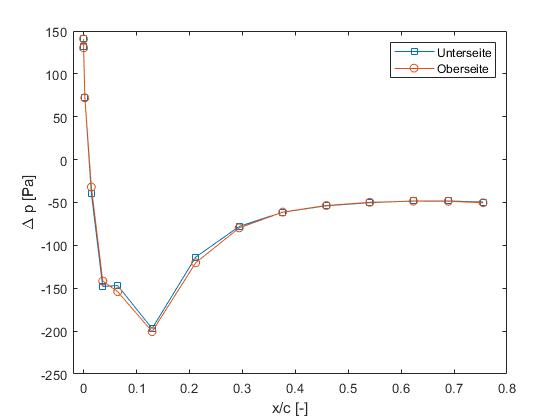
\includegraphics[width=0.6\textwidth]{Oberflaechendruecke_RK.jpg}
	\caption{Oberfl"achendr"ucke bei der eingebauten Basiskonfiguration}
	\label{fig:Oberflaechendruckverteilung RK}
\end{figure}

Aus \abb{fig:Oberflaechendruckverteilung RK} ist ersichtlich, dass die Druckdaten auf Ober- und Unterseite nur kleine Abweichungen im Bereich von bis zu 3\,\% aufweisen.\\
Diese Abweichung liegt im Bereich der Messungenauigkeiten und ist somit tolerabel.
Mittels dieser Messung ist also festgestellt, dass das Modell symmetrisch in der Antr"omung steht und die Versuchsreihen mit der Basiskonfiguration k"onnen durchgef"uhrt werden.

Um die periodische Aktuation zu erm"oglichen, werden die glatten, zylindrischen Wellen aus Aluminium nach diesen Versuchen gegen die in \abschn{s:rotierendeWalzen} beschriebenen, ovalen Wellen getauscht.

Anschlie\ss{}end an den Einbau wird erneut die Druckverteilung auf der Oberfl"ache des Modells gemessen, um eine optimale Postion des Modells ohne Anstellwinkel zu gew"ahrleisten. Die Ergebnisse sind in \abb{fig:Oberflaechendruckverteilung 50}
zu sehen.

	\begin{figure}[h]
	\centering
	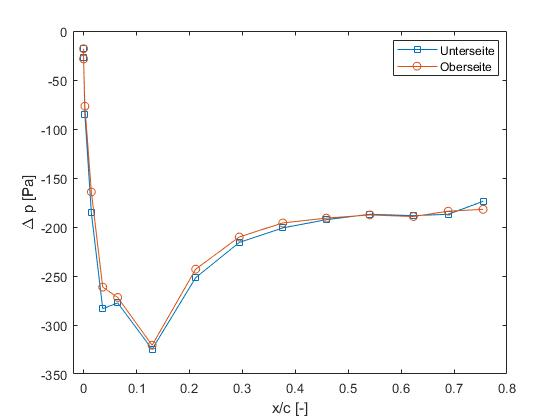
\includegraphics[width=0.6\textwidth]{Oberflaechendruecke_50erK.jpg}
	\caption{Oberfl"achendr"ucke beim eingebauter Konfiguration 50}
	\label{fig:Oberflaechendruckverteilung 50}
	\end{figure}

Die Dr"ucke an der Ober- und Unterseite sind hier wieder gespiegelt und "ubereinandergelegt dargestellt. Der erste Messpunkt entspricht dabei der Druckmessbohrung, die mittig an der Vorderseite eingebracht ist.

Die gr"o\ss{}te Abweichung erf"ahrt der Druck an Ober- und Unterseite genau dort, wo auf beiden Seiten das Zackenband angebracht wurde. Der lokale, jeweilige Abstand der Druckmessbohrung zum Zackenband ist allerdings oben und unten nicht komplett einheitlich. Dies hat zur Folge, dass das Str"omungsverhalten an diesen Orten voneinander abweicht, wodurch die Differenz zu erkl"aren ist.\\
Zu bemerken ist, dass das Zackenband auf die Oberfl"achendr"ucke der Basiskonfiguration keinen gro\ss{}en Einfluss hat. M"oglicherweise ist bei den Schritten, die zwischen diesen beiden Messungen liegen, das Zackenband leicht in der Position beeinflusst worden.

Da die Druckmessbohrungen im Folgenden keine gro\ss{}e Relevanz haben, ist diese Ungleichm"a\ss{}igkeit kein Problem.

Weiterhin ergibt sich allerdings im Unterschied zu den Messungen der Oberfl"achendr"ucke an der Basiskonfiguration eine leichte Druckerh"ohung an der Oberseite zur letzten Druckmessbohrung hin.
Auch in der Arbeit von \emph{Bilges} \,\cite{Bilges.2018}, die das gleiche Modell als Gegenstand der Untersuchung hatte, ist eine "ahnliche Entwicklung bei niedrigeren Reynoldszahlen als 50.000 zu sehen gewesen.
Die beschriebene Tendenz war aber bei h"oheren Reynoldszahlen wieder kaum wahrnehmbar.


Diese Erscheinung lie\ss{} sich auch nach "Uberpr"ufung der Schl"auche und Bohrungen auf Verunreinigungen bzw. Verstopfungen und mehreren Nachjustierungen der Modellpostion nicht beseitigen.\\
Auch der m"ogliche Einfluss der oberen und unteren Walze auf diese Werte durch etwaiges leichtes Aufbiegen der Spalte in variierenden Walzenstellungen wurde ohne positive Ver"anderung getestet.

Das Auseinanderstreben der Messwerte ist somit wahrscheinlich auf die in \cite{Bilges.2018} angef"uhrten einseitigen Fertigungstoleranzen und Unebenheiten zur"uckzuf"uhren, welche je nach individueller Einstellung der Spalte bei den verschiedenen Walzenpaaren unterschiedlich stark zum Vorschein kommen.

Da an den anderen Messpunkten Ober- und Unterseite sehr "ahnliche Werte liefern, kann trotz dessen davon ausgegangen werden, dass das Modell symmetrisch in der Anstr"omung platziert ist.


%Die eigentlichen Messreihen gestalteten sich bei dieser Konfiguration aus verschiedenen Gr"unden als schwieriger und aufw"andiger als bei der Konfiguration aus \abschn{sec:ErgebnisseKonstanteAktuation}.

%Damit lokale
%
%Phasenungleicheit bei der Wellenrotation.:
%
%Da nicht ausgeschlossen werden kann, dass die beiden Walzen beim Hochfahren der Drehzahl asynchron laufen und sich eine phasenversetzte Aktuation an Ober- und Unterseite ergibt, wurden zu jeder Kombination der Messparameter mehrere Messungen durchgef"uhrt.
%
%Eine 